\documentclass[sigconf]{acmart}

\usepackage{booktabs} % For formal tables
\usepackage{framed}
\usepackage{color}
\usepackage{caption}
\usepackage[font=small]{subcaption}
\usepackage{multicol}

% Copyright
%\setcopyright{none}
%\setcopyright{acmcopyright}
%\setcopyright{acmlicensed}
\setcopyright{rightsretained}
%\setcopyright{usgov}
%\setcopyright{usgovmixed}
%\setcopyright{cagov}
%\setcopyright{cagovmixed}


%Conference
\acmConference[MOCO '18]{5th International Conference on Movement and
Computing}{June 2018}{Genoa, Italy}
\acmYear{2018}
\copyrightyear{2018}

\settopmatter{printacmref=false}

\newenvironment{Figure}
  {\par\medskip\noindent\minipage{\textwidth}}
  {\endminipage\par\medskip}

\begin{document}


\title{Improv: Live Coding for Robot Motion Design}


%\author{Alexandra Q. Nilles}
%\orcid{1234-5678-9012}
%\affiliation{%
%  \institution{Computer Science Department \\ University of Illinois at
%Urbana-Champaign}
%}
%\email{nilles2@illinois.edu}
%
%\author{Chase Gladish}
%\affiliation{%
%  \institution{Computer Science Department \\ University of Illinois at
%Urbana-Champaign}
%}
%\email{webmaster@marysville-ohio.com}
%
%\author{Mattox Beckman}
%\affiliation{%
%  \institution{Computer Science Department \\ University of Illinois at
%Urbana-Champaign}
%}
%\email{larst@affiliation.org}
%
%\author{Amy LaViers}
%\affiliation{%
%  \institution{Mechanical Science and Engineering Department \\ University of Illinois at
%Urbana-Champaign}
%}

% The default list of authors is too long for headers.
%\renewcommand{\shortauthors}{A. Nilles et al.}

\begin{abstract}
This paper introduces the Improv system, a programming language for high-level
description of robot motion with immediate visualization of the
resulting motion on a physical or simulated robot. The intended users of this
tool are anyone looking to quickly generate robot motion, such as educators,
artists, and researchers. The system includes a domain-specific language,
inspired by choreographic techniques, which allows for several ways of composing
and transforming movements such as reversing movements in space and time and
changing their relative timing. Instructions in the Improv programming language
are then executed with \emph{roshask}, a Haskell client for ROS ("Robot Operating
System"). ROS is an open-source robot software framework which is widely used in
academia and industry, and integrated with many commercially available robots.
However, the ROS interface can be difficult to learn, especially for people
without technical training. This paper presents a "live coding" interface for
ROS compatible with any text editor. Currently, Improv can be used to control any robot compatible with the
`Twist' ROS message type (which sets linear and rotational velocity). This paper
presents Improv implementations with the two-dimensional simulator
Turtlesim, as well as three-dimensional TurtleBots in the Gazebo simulation
engine.
\end{abstract}


%
% The code below should be generated by the tool at
% http://dl.acm.org/ccs.cfm
% Please copy and paste the code instead of the example below.
%

\keywords{robotics, choreography, live coding, ROS, Haskell, roshask, HRI}


\maketitle


\section{Introduction}\label{introduction}

Robotic technology is becoming more commonly integrated into settings outside of
the factory - including classrooms \cite{mataric2004robotics} and art installations
\cite{kukaDance2017}. There
is also an increasing need for robotic technology in research labs and
workplaces for automating repetitive or uncomfortable tasks, in which case
users often only need to specify a few simple movements. All of
these applications would benefit from a method of programming robots that is
faster and more high-level than the current workflow.


Currently, many commercially available robots are programmed through proprietary
interfaces (which may be graphical, text-based, or physically interactive) or through ROS (the "Robot Operating System,"
a middleware and collection of libraries which manages message passing between
the many components of robot systems) \cite{rossano2013easy}
\cite{quigley2009ros}. However, this
workflow has two obstacles that often make robot programming difficult,
especially for newcomers to the field. First, the programming languages and
interfaces are
often at a low level of abstraction, forcing users to translate their
mental model of their intended movement, often introducing
mistakes and frustration. Second, the process of writing code, compiling and
executing the instructions on the robot platform can be time-intensive and
requires the user to switch between several different software modalities (text
editor, to command line, to simulation software or hardware platform).

The tool introduced in this paper, \emph{Improv}, addresses both of these
problems. To address the first (mismatch between the problem and
program domains), we introduce a small domain-specific programming language
(DSL) with motion primitives and several operators which allow
movements to be combined and transformed, in space and time. The transformations
are inspired by choregraphic techniques, such as those in
\cite{laviers2017choreographic} \cite{cuykendall2014designing} \cite{alaoui2014choreography} and
\cite{humphrey1959art}.


For example, the following ROS Python client code will cause a
mobile robot such as a Roomba or Turtlebot to follow a path that curves
forward and left:

\begin{verbatim}
if __name__ == '__main__':
    pub = rospy.Publisher('turtle1/cmd_vel',Twist)
    rospy.init_node('publisher_node')
    loop_rate = rospy.Rate(5)
    while not rospy.is_shutdown():
        vel=Twist()
        vel.linear.x = 1.0
        vel.angular.z = 1.0
        pub.publish(vel)
        loop_rate.sleep()
\end{verbatim}

while the equivalent code in \emph{Improv} is

\begin{verbatim}
turtle1 $ forward || left
\end{verbatim}

where $||$ is an operator which combines movements in parallel.

To address the second obstacle to robot programming (the difficult
process of evaluating code on a robot), we introduce a "live coding"
infrastructure: when changes to the program file are saved, the process of
interpreting code and converting high-level commands to low-level ROS messages
is done automatically and the user can observe the effects on the simulated or
physical robot nearly immediately.

By addressing these two shortcomings of current robot programming tools, we hope
to make robotics more accessible and usable for a broader range of people,
not just expert roboticists. Possible users of this tool include
artists, educators, newcomers to robotics, and anyone who wishes to quickly
prototype robot motion patterns. \emph{Improv} is open-source and available at
\emph{[redacted]}
%\url{https://github.com/alexandroid000/improv}
. Please let us know if you try it
out!

\subsubsection*{Related Work}

We are aware of two other projects addressing the problem of the complex
development cycle in ROS by creating tools for interactive or ``live''
programming. One such project \cite{python_live_DSLRob} created a DSL in Python
which allows for wrapping and modifying existing ROS nodes, using the Python
shell. However, by using the Python shell, the user is only able to experiment
with commands in a shell and is not able to save the commands they have tried in
a file. Additionally, since the DSL is implemented as a library in Python, it
inherits some of the opaque syntax of the Python ROS client. Improv has a
simpler, albeit less powerful, programming language and models movement
explicitly. Another closely related work to \emph{Improv} is the Live Robot
Programming (LRP) language \cite{campusano2017live} and its integration with PhaROS
\cite{estefo2014towards}, a client library for ROS written is Pharo, a dynamic
programming language specialized for live updating and hot recompilation. This
project allows for live coding of ROS nodes and reconfiguration of the ROS
network with a much shorter development cycle than traditional ROS programming.
However, the aims of these projects and Improv are different - the LRP DSL,
while more high-level than most robot programming languages, was not designed
around modelling movement itself and instead models state machines that
transition on events. Both of these related projects are better suited for
applications which involve reactivity and sensing of the environment, while
Improv is better suited to applications where the user wishes to quickly
generate certain movements and creatively explore movement patterns.

This work is also heavily influenced by live coding interfaces and programming
languages for generating music and visuals, which are often associated with the
Algorave performance movement \cite{collins2014algorave}. In particular, the
programming language TidalCycles \cite{mclean2010tidal} has had a strong
influence on this work, both syntactically and in how relative timing of events
is managed. \emph{Al Jazari} is a live coding installation which uses a simple
graphical language to allow people to control robots (in simulation)
\cite{mclean2010visualisation}. The language includes conditionals based on
external state and communication between the bots. The program state of the
robot is also visualized. There are a variety of other projects centered around
live coding interfaces for controlling cyberphysical systems and visual
simulators, such as Extempore and integrations of TidalCycles with Unity3D
\cite{livecoding14}. These initiatives are often more purely focused on
performance than \emph{Improv}, and as far as we know, none are compatible with
ROS.

In the robotics space, another closely related project to \emph{Improv} is \emph{Dance}, a
domain-specific language built in Haskell \cite{Dance2003}. The project includes
a DSL inspired by Labanotation, as well as a reactive layer that allows the
robot to respond to sensor events. The project targets humanoid robots, while
\emph{Improv} has so far targeted mobile robots, and \emph{Dance} would generate
the necessary 3D simulation code, though did not include the live coding
interface of this work and predates ROS. \emph{Improv} has incorporated and
adapted some of the data structures from \emph{Dance}, namely the
\texttt{Action} and \texttt{Dance} data types. Another relevant project is
\emph{roshask} \cite{cowley2011stream}, a Haskell client library for ROS, which
this project uses as an interface between our domain-specific language and ROS.
Some relevant design features of \emph{roshask} will be described in Section
\ref{interfacing-with-ros}. Especially when used with the two-dimensional Turtlesim, \emph{Improv}
is reminiscent of \emph{Logo} \cite{logo}, an educational, interpreted
dialect of Lisp that is often used in conjunction with a simulation of a
two-dimensional turtle. Our programming language is less expressive and powerful 
than \emph{Logo}, but is integrated with ROS and thus able to be used with
three-dimensional simulators and actual robots.

\subsubsection*{Paper Outline}

Section \ref{embodied} details how this work was inspired by embodied
improvisation for robot motion design, as well as concepts from the field of human-computer
interaction, and the resulting design principles for the tool.
Section
\ref{architecture-overview} provides an overview of the software architecture,
how the features of \emph{Improv} implement
our design principles, and some example programs. Section
\ref{domain-specific-language-design} describes some of the design decisions and
features of the high-level domain-specific language, as well as the
corresponding design choices in the Haskell backend. 
Section \ref{interfacing-with-ros} details more about how ROS messages are
defined for specific robotic platforms, and how the live coding interface is
implemented. Finally, Section
\ref{conclusions-and-future-work} summarizes our conclusions and outlines directions
for future work, including user studies.



\begin{figure*}
 \centering
\includegraphics[width=0.9\textwidth]{/home/alli/common/figs/rosfig.jpg}
\captionof{figure}{An example of a typical workflow in ROS, created by following a
beginner tutorial. There are five overlapping terminal windows open, as well
as the Gazebo simulator. \label{rosfig}}
\end{figure*}



\section{Prototyping Movement Design in Embodied Improvisation}\label{embodied}

\emph{Improv} is a tool for \emph{prototyping} robot motion. Put another way, it
is a tool for improvising movement on robot platforms. The authors have taken
inspiration from their experiences with embodied improvisation, which is often
used by choreographers and dancers as a way of understanding and creating human
movement. Experts such as William Forsythe have analyzed strategies for
improvisation for choreography and performance \cite{forsythe2004improvisation}.
Improvisation helps the movement designer understand and explore the plethora of
movement options that are available at any given time. This is especially useful
in robotics applications as the field starts to explore stylized movement and
the incorporation of robotic technology into homes and artistic performances. For
example, one may explore different ways of picking up a cup (as if one is
underwater, or as if one is being electrocuted, or in the style suggested by
different pieces of music) in order to understand how many different ways there
are for a robot to perform one task, and the percieved effects of all these
different motion strategies.

However, the time taken to set up environments and write, compile and
execute code often negates the benefits of improvisational practice when done
on a robotic platform instead of a human body. This is
doubly true when working with robotic hardware, and these barriers especially
affect those users who do not have a strong background in programming. This places
some design constraints on the \emph{Improv} system - namely, the system must
have

\begin{itemize}
\item a minimal ``representational
distance" between the user's mental model of the movement they want to try and
the description in code, so there is minimal frustration and time wasted in
translation,
\item a near-imperceptible delay between writing instructions to the robot and
seeing the effect of those instructions, and
\item a singular environment where the
user interacts with the program (to avoid the user's attentional flow being
broken by needing to switch between different interaction modalities).
\end{itemize}

These and similar design principles have been thoroughly studied in the field
of human-computer interaction. In particular, the authors were inspired by several of the principles
outlined in the `cognitive dimensions of notations' \cite{green1996usability}.
There are eleven `cognitive dimensions,' or design principles, that the authors
describe but several are especially relevant to this work, such as

\begin{itemize}
\item \emph{Closeness of mapping}: What `programming games' need to be learned?
\item \emph{Diffuseness}: How many symbols or graphic entities are required to express a meaning?
\item \emph{Error-proneness}: Does the design of the notation induce `careless mistakes'?
\item \emph{Hard mental operations}: Are there places where the user needs to resort to  fingers or pencilled annotation to keep track of what's happening?
\item \emph{Progressive evaluation}: Can a partially-complete program be executed to
obtain feedback on `How am I doing'?
\end{itemize}

Designing \emph{Improv} with these principles in mind has helped us minimize the mental
load of using the tool, and enable faster prototyping and a more
improvisational workflow.


\section{Improv Architecture and Features}\label{architecture-overview}

See Figure \ref{flowchart} for a diagrammatic representation of
the components in the \emph{Improv} system and their relationships.

Several design features have been chosen to
address the design constraints in Section \ref{embodied} (rapid development
cycle, more natural translation of movement to code, and a single user environment).
These design choices were made in part due to the usual workflow in ROS. For
example, a beginner tutorial for ROS will have the user open at least three
terminal windows (one for starting the ROS server, one for starting a
publishing node, and one for starting a subscriber or simulator) and an editor,
for a total of five windows (including the simulator). This process can be very
intimidating for people who may not have experience with Linux or the command
line, and the multitude of windows and interaction modalities make it difficult
for the user to have a coherent mental model of information flow in the system.
It is often not possible to see all the relevant windows at one time on a
regular computer monitor. See Figure \ref{rosfig} for an example.

Despite its lack of user amenities, ROS is a very powerful tool - it is
integrated with many commercially available robot platforms, and includes many
libraries for standard robot use cases. Thus, we have chosen to design
\emph{Improv} as a wrapper around ROS. This gives us the benefits of ROS's
infrastructure, but we exchange the powerful low-level control available in
most ROS client libraries for the simplicity of a high-level representation of
robot motion.
To specifically address the design criteria in Section \ref{embodied}, we have
included the following features in \emph{Improv}:

\begin{itemize}
\item \emph{small representational distance between
movement and code:} a domain-specific language, inspired by choreographic
techniques such as spatial symmetries, relative timing changes, and body-centric
coordinates. Many domain-specific languages for robot programming exist; for example, a
review in 2016 identified 137 relevant publications 
\cite{nordmann2016survey}. However, most model robotic
systems from a control-flow perspective, and do not model motion directly. The
desired language will depend heavily on the programmer's task, but undoubtably
there are many applications where users would like to describe the robot's
instructions directly in terms of movement. It then makes sense to directly use
the expertise and terminology developed by choreographers and other movement
experts. 
\item 
\emph{rapid movement prototyping:} changes to the user's file are interpreted by a 
Haskell program that builds a ROS node for publishing messages to a
simulator or physical robot. This process is nearly real time, allowing for a
seamless user experience.
\item \emph{workspace with few attentional switches:}
a live coding interface with only two windows, one for editing the text file and
one for observing effects on a simulated robot. Currently, we have tested the
system with:
\begin{itemize}
  \item
    TurtleSim: a two dimensional simulator where
    velocity commands nearly perfectly control an animated turtle.
  \item
    Gazebo with a TurtleBot robot model: a three-dimensional simulator
    with more realistic physics, where velocity commands control
    simulated motors.
  \end{itemize}
\end{itemize}

\begin{figure}[h]
\centering
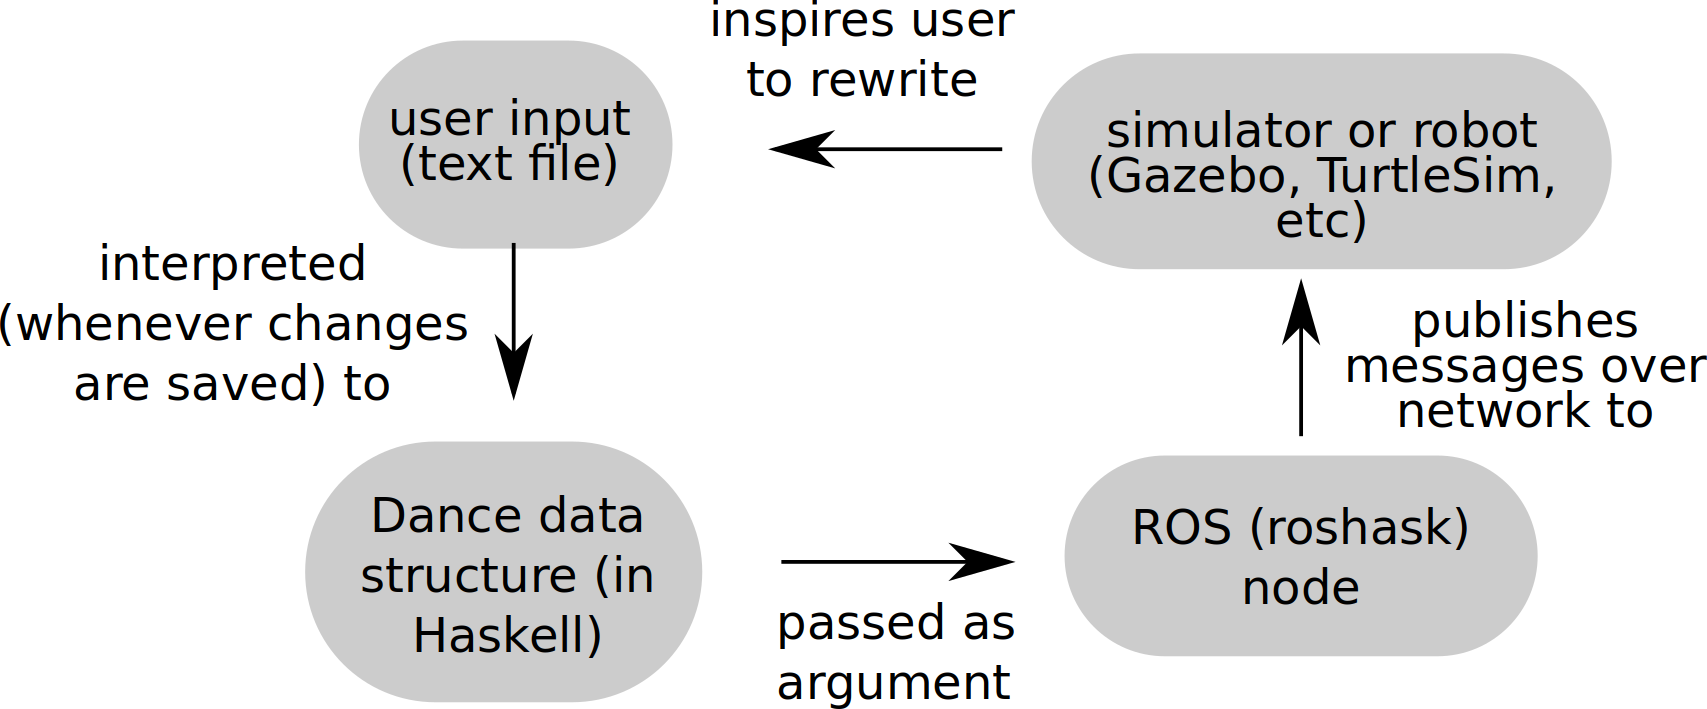
\includegraphics[width=8.00000cm]{/home/alli/common/figs/flowchart.pdf}
\caption{An illustration of how user input, written to a text file, is
converted into a ROS node which publishes messages to a simulator or physical 
robot.
\label{flowchart}}
\end{figure}


\begin{figure*}[h!]
    \begin{subfigure}{0.45\textwidth}
        \includegraphics[width=8cm]{/home/alli/common/figs/improv_gedit_gazebo.png}
        \captionof{figure}{A program as it appears in Gedit, a simple graphical text editor, with
        the physics-based simulator Gazebo and a simulated
        Turtlebot.\label{gedit}}
    \end{subfigure}\hfill%
    \begin{subfigure}{0.45\textwidth}
        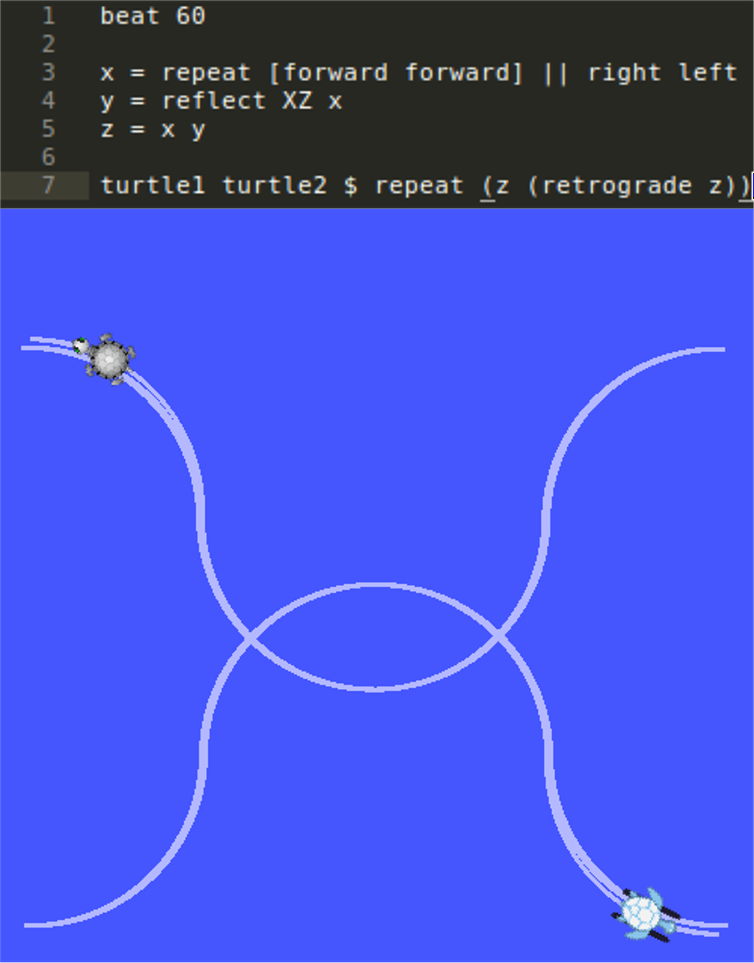
\includegraphics[width=8cm]{/home/alli/common/figs/termturtle.png}
        \captionof{figure}{A program as it appears in vim, a terminal-based text editor, with the
         resulting movement in TurtleSim on two
        simulated turtles.\label{vim}}
    \end{subfigure}
    \caption{Examples of different text-editor and simulation environment
configurations available to users of \emph{Improv}. Any text editor can be
used, while simulators or robots must be compatible with the ROS message types
implemented with the system.}
\end{figure*}



The first feature, the domain-specific language, corresponds to the cognitive
dimension \emph{closeness of
mapping}. As Green and Petre described, "the closer the programming world is to
the problem world, the easier the problem-solving ought to be. Ideally, the
problem entities in the user's task domain could be mapped directly onto
task-specific program entities, and operations on those problem entities would
likewise be mapped directly onto program operations" \cite{green1996usability}.
This also helps along the dimension of \emph{diffuseness}: as the example in the
introduction showed, we are able to express a movement such as curving forward
and left very concisely, without cluttering the code space with the low-level
infrastructure requirements of most ROS client libraries. Less noisy code also
helps with \emph{error-proneness}, since the user does not need to manually
configure as many settings. We have also tried to make our parser flexible, by
allowing different amounts of whitespace between lines and operators, though
this area could certainly use more improvement. The final two features, the fast
compile time and simple user environment, both help reduce \emph{hard mental
operations} and gives the user a fast and easy way to use \emph{progressive
evaluation}.

All of these features are intended to give the user a sense of \emph{flow}: a
mental state of complete absorption in the activity. The fewer distractions and
focus changes in the activity, whether it is improvisational dance or coding,
the higher the chance of the participant becoming completely engaged and
accessing all the creative options available.


As examples of possible user interfaces, Figures \ref{gedit} and \ref{vim} show examples of the system in use with two
different text editors and two different simulators. Note that the choice of
editor and the choice of simulator are decoupled, and \emph{Improv} is
absolutely editor-agnostic, relying only on an operating-system level script
to execute changes. \emph{Improv} is somewhat simulator-agnostic: 
currently it is only possible to control robots which use a \texttt{Twist} ROS messages
for control, which set desired linear and rotational
velocities.


\section{Domain Specific Language (DSL)
Design}\label{domain-specific-language-design}


The base type of the \emph{Improv} language is a movement. Movements are
discretized and can be combined with each other in various ways, forming new
movements, which can be in turn transformed and combined. The precise way in
which this is interpreted on a robot platform is defined by the language's
translation to Haskell and the resulting messages sent over the ROS network,
which will be described further in Section \ref{interfacing-with-ros}.


\begin{figure}[h]
\centering
\begin{verbatim}
prim = rest  | forward 
     | left  | halfleft
     | right | halfright

transformer = reverse  | retrograde 
            | repeat n | reflect ax

movement = prim
         | movement movement
         | [movement]
         | (movement)
         | movement || movement 
         | transformer movement

exp = rs $ movement
    | var = movement
    | beat n
\end{verbatim}
\caption{The grammar of Improv programs. \texttt{exp} represents top-level
expressions, which execute movements on robot(s), or store movements in
variables. \texttt{movement}s are converted into ROS message streams and can be
composed and grouped in multiple ways. \label{grammar}}
\end{figure}

Figure \ref{grammar} shows the grammar of the \emph{Improv} language.
The language supports primitives such as \texttt{forward} and \texttt{right}
corresponding to commands to the robot causing it to perform the expected
motion. These primitives are composed in series, sequence and parallel, and
transformed in time and space.

Movements are organized in time into units, where each unit is performed in one
``beat.'' The base timing of beats (units per minute) can be specified by the
user, and is only limited by the maximum publishing frequency of ROS and the
physical constraints of the robot platform.

Users can specify a series of commands such as \emph{move forward for
one beat, turn right for one beat, move forward for one beat} with the
command \texttt{forward right forward}. Movements separated by whitespace 
on the same line will occur in different ``beats.''

The user can also use brackets to compress a sequence of movements into
one beat, such as \texttt{[forward right forward]}, which will
cause these three movements to happen in the same amount of time as the
first movement in the previous example. This syntax and behavior is directly 
inspired by \emph{TidalCycles}, which has a similar mechanism for grouping
sounds. In our implementation,
bracketing $n$ movements causes each movement to be performed $n$
times faster, but for $1/n$ times as long, so the movement has the
same spatial extent but is performed faster.

Movements can also be performed in parallel, such as
\texttt{forward \textbar{}\textbar{} right}, which will cause the
robot to curve to the right as it moves forward. In our implementation,
velocities in parallel are simply added, so
\texttt{left \textbar{}\textbar{} right} would result in no
movement. Movements in parallel will terminate
when the ``shorter'' movement ends, so the program
\texttt{(forward right) \textbar{}\textbar{} forward} will never turn
right (parenthesis are used to group movements without changing timing).

We have also implemented several transformations which map a function
over a movement. For example, \texttt{repeat} takes an integer and a
movement as arguments and causes that movement to repeat for the
specified number of times.

In space, we have \texttt{reflect}, which takes a plane and a movement
as arguments and returns the reflected movement
(\texttt{reflect\ YZ\ right} yields \texttt{left}, where the \texttt{YZ}
plane is body-centered and could also be called the saggital plane). For transforming movements in time, \texttt{reverse} is a
unary operator which will reverse the order of a series of movements:
\texttt{reverse\ (forward\ right\ left)} is equivalent to
\texttt{left\ right\ forward}. To reverse the trajectory itself, we use
\texttt{retrograde}, which uses spatial reflections and reverses time;
for example, \texttt{retrograde\ (forward\ right\ left)} is equivalent
to \texttt{right\ left\ backward}. Both \texttt{retrograde} and
\texttt{reverse} are their own inverses: applying them twice returns the
original movement, as would be expected.

While we have only implemented these combinators for simple and very
symmetric mobile robots, one could imagine making more complicated types
of symmetry for other robot platforms. We have included a typeclass
\texttt{Symmetric\ a}, parameterized by a body type \texttt{a}, and defined by a function
\texttt{refl\ ::\ Plane\ -\textgreater{}\ a\ -\textgreater{}\ a}. By defining this
typeclass once for a new robot platform, detailing all the different symmetries of
the body, the functionality of these spatial transformers can be
extended to new platforms.

\subsection{Multiple Robots}\label{multiple-robots}

The \emph{Improv} system has the capapbility to control multiple robots
at once, using a syntax which mirrors how \emph{TidalCycles} allows for
multiple tracks to be played simultaneously. Each robot is given a
unique name in the shell script which launches ROS and the \emph{Improv}
system (this is also where the initial location of each robot is
specified). Then, in the user's program, they specify which movement
sequence should be associated with each robot. For example, to make
robot \texttt{r1} move forward and robot \texttt{r2} move backward, the
user would write

\begin{verbatim}
r1 $ forward
r2 $ backward
\end{verbatim}

This syntax, along with assigning movements to variables, can make it easy to
specify relationships between how different robots are moving, such as

\begin{verbatim}
x = left right [forward right]
r1 $ x
r2 $ retrograde x
\end{verbatim}


which would cause robot \texttt{r2} to perform the same movement as
robot \texttt{r1}, but in retrograde. It is also possible to command two robots
to do the same movement with a program such as

\begin{verbatim}
r1 r2 $ forward backward
\end{verbatim}

As \emph{Improv} is extended to other platforms in the future, this could be an
interesting mechanism for studying how the same high-level choreographic
commands are perceived when executed on different platforms.

\subsection{Modelling Movement in
Haskell}\label{modelling-movement-in-haskell}

Programs in the \emph{Improv} DSL are interpreted by a compiled Haskell
program into an abstract data type (ADT), which represents each
\texttt{movement}. This ADT, which we call a \texttt{Dance}, can be thought of as
a tree that holds all movement primitives and their compositions and
transformations. To
execute a \texttt{Dance} as a series of ROS messages, we must flatten
the tree while maintaining their relative timing information, which will
be discussed in Section \ref{relative-timing}.

\texttt{Dance}s are defined as

\begin{verbatim}
data Dance b = Prim Action Mult b
             | Rest Mult
             | Skip
             | Dance b :+: Dance b
             | Dance b :||: Dance b
\end{verbatim}

where \texttt{Prim} is a motion primitive type, composed of the
\texttt{Action} (direction and spatial extent of the movement),
\texttt{Mult} which stores timing information, and \texttt{b}, a parameterized type describing the
part of the robot to move. \texttt{Rest} indicates that the robot part
is not moving for some period of time (and is a primitive in the
\emph{Improv} language). 

\texttt{Skip} is the identity dance, having no
effect on the robot for no time duration, and is necessary for the
monoidal structure of the parallel and
series operators (\texttt{:\textbar{}\textbar{}:} and \texttt{:+:},
respectively), which are binary operators on \texttt{Dance}s.

This algebraic structure helps enforce the timing behavior that we
expect; namely, associativity. If \texttt{d1}, \texttt{d2}, and
\texttt{d3} are all \texttt{Dance}s (with an arbitrary number and
structure of movement primitives in each), then we want to ensure the
following equivalence:

\begin{verbatim}
(d1 :+: d2) :+: d3 = d1 :+: (d2 :+: d3).
\end{verbatim}

Similarly, if three \texttt{Dance}s are in parallel, arbitrary groupings
should not change the meaning of the program. This is exactly the
behavior that the algebraic objects \emph{monoids} have: 
associativity and an identity element. See \cite{yorgey2012monoids} for a much more
detailed discussion on the usefulness of monoids in modelling and
programming languages, in the context of \emph{Diagrams}, a Haskell DSL
for creating vector graphics.

We create monoid instances in Haskell for these operators on
\texttt{Dance} data types, which allow for lists of \texttt{Dance}s to be combined
in sequence or parallel. This is useful because the parser returns expressions
in the user's program as a list of \texttt{Dance}s. By implementing our intuitive understanding that movements in parallel and
series should be associative as an algebraic structure, we can use the power of Haskell's abstractions to
get the correct behavior ``for free."

Similarly, we use the Haskell functionality for mapping functions over data structures
(such as our \texttt{Dance} trees) to implement transformers such as
\texttt{retrograde} and \texttt{reverse}. We define these functions recursively
over the \texttt{Dance} ADT, by first defining a function \texttt{transform}
which has two arguments: the first, a function transforming individual
\texttt{Action}s (for example, flipping them over a spatial axis, or shrinking
their extent), and the
second being a \texttt{Dance}. The \texttt{transform} function then returns the
transformed \texttt{Dance}. This allows us to abstract out transformations from the
low-level details of how they are propagated through the ADT, making it easier
to implement new transformers.

\subsection{Relative Timing}\label{relative-timing}

As programs are parsed and converted to ROS messages, we must enforce the timing semantics - for example, movements
inside square brackets, such as \texttt{{[}forward\ right\ forward{]}},
must occur within one ``beat.'' The parser returns such a program as a list of \texttt{Dance}s, labelled with a type
that indicates that they should be compressed in sequence.
Then we call a function \texttt{seqL} which uses the length of the
 list to determine how much to speed up each individual dance
before composing the movements. This is accomplished with a function
\texttt{changeTiming} which takes a multiplier \texttt{m} and a
\texttt{Dance}, and propagates the multiplier through the \texttt{Dance}
recursively. This allows for nested sequential movements: for example,
the program \texttt{{[}forward\ {[}left\ left{]}\ forward{]}} would
result in timing multipliers \texttt{[3, 6, 6, 3]}. Note that the \texttt{left}
primitives will have \texttt{Mult}s of 6, since
they must occur six times as fast as normal to allow the whole movement
to occur in one ``beat.'' Thus, movements are able to be arbitrarily sped up by
placing them in sequence inside square brackets. Movements can only be slowed
down by decreasing the \texttt{beat} parameter in the program file, which sets
the number of time units per minute. By making this number smaller, movements
such as a quarter turn will be slowed down to fill the specified unit of time.
Future work may include a language primitive which is able to do this for
smaller chunks of code inside the program file, instead of needing to change the
global timing parameter.

\section{Interfacing with ROS}\label{interfacing-with-ros}

\emph{Roshask} is a client library for ROS, written in Haskell. It treats streams of values (such as those published
and subscribed to by ROS nodes) as first class values, which allows for them to
be combined and transformed in more natural ways than imperative ROS client
libraries. For example, when we put \texttt{Dance}s in parallel, we wish to combine two
lists of motion commands with some function for parallel execution - whether this
is averaging commands which affect the same body part, or additively combining
them, or whatever interpretation the designer wishes for a specific robot
platform. In Haskell, this is accomplished easily with the
\texttt{zipWith} function, which takes two lists and a function for combining values in
those lists. \emph{Roshask} extends this expressivity to the combination and
transformation of ROS message streams, making it a useful tool for implementing
the \emph{Improv} DSL.

The primitives in \emph{Improv}, such as \texttt{forward} or \texttt{right}, are
mapped to streams of ROS messages. In our implementation so far, we have mapped
to the \texttt{Twist} ROS message, which specifies the robot's linear and
angular velocity as two three-dimensional vectors. Velocity controllers, which
often are included with commercial robots, are required to create the low-level
motor controls for reaching and maintaining the desired velocities. 

To integrate a robot with \emph{Improv}, one must
specify how to convert the \texttt{Dance} data structure to a list of ROS
messages. For example, for a non-articulated symmetric mobile robot (such as a Roomba or
TurtleBot), this is accomplished by two functions: \texttt{moveBase} and
\texttt{danceToMsg}. Since the robot has only one body part, \texttt{moveBase}
takes an \texttt{Action} (direction and extent of movement) and converts it to a
single ROS velocity command (which sets the desired linear and rotational
velocity in the plane). 
Here, we have simplified the language
by varying only three velocity values, the robot's \(x,y-\)velocity in
the plane and its angular velocity in the plane.

Since our discretization of movements is relational (for
example, you can have \texttt{Full}, \texttt{Half}, and \texttt{Quarter} extent,
and directions are related through symmetries), only a small number of these
translations from \texttt{Action}s to velocities need to be explicitly defined
and the rest can be derived through their relations. For example,
\texttt{moveBase (A dir Half)} is defined as \texttt{fmap (*2) (moveBase (A dir
Quarter))},
where \texttt{fmap} maps the function \texttt{*2} over the values in the velocity
command returned by \texttt{moveBase (A dir Quarter)}. This encodes the relationship
that a \texttt{Half} extent is twice as far as a \texttt{Quarter}, thus the
robot must move twice as fast in the same direction to travel twice the distance
in the same amount of time. Defining these relationships explicitly helps speed
up recalibration or extension of the platform to new robots and simulators -
onwith mappings from \texttt{Dance}s to ROS messages need to be hard coded,
and the rest are derived from the relations.

Once this conversion (from a \texttt{Dance} data structure to a list of ROS messages)
has been completed, the list of ROS messages is passed to a ROS
node defined in \emph{roshask}. This node publishes the commands over the ROS network.
Even if multiple robots are controlled, the system still only uses one ROS node
which publishes to multiple topics. Work is ongoing on whether to extend the
system to control multiple ROS nodes, and if so, how best to implement this
feature.

\subsection{Live Coding Interface}\label{live-coding-interface}

One important design decision for developers of interactive text-based
programming tools is whether to tie their tool to a specific editor. For
example, the live coding tool TidalCycles was originally
developed for Emacs, a powerful editor which has a notoriously steep
learning curve. Many people prefer to use simpler editors, so new
live coding plug-ins have been developed for editors such as Atom and
Sublime Text. This editor-based approach has advantages, such as a large
degree of customizability and extensibility using the features of the
editor. However, it also introduces challenges such as maintaining
feature parity between editors, as well as the up-front investment
needed to interface with new editors. In our case, we are developing a
tool that should be usable by artists, children, and programming
novices, as well as experienced roboticists. Thus, we wish to allow
users flexibility to choose their editor of preference.

To accomplish this, instead of creating an interface for each desired
editor, we use a shell script which monitors the file that the user is
editing for changes. Every time the user saves changes to the file, the
program detects a change, interprets the user's new program, and resets
the simulator and ROS node. This design choice circumvents the need to
interface with specific editors. Additionally, many editors have
keyboard shortcuts for saving files. Thus, executing programs
contributes minimally to the overall workload of using the system,
especially when compared to the many steps required to test changes to
traditional ROS programs. The delay between saving the file and observing the
changes in the simulator is very short - while we have not done a formal timing
analysis, the delay is a small fraction of a second and not noticeably longer than the
time it takes to look from the text editor to the simulator.

\section{Conclusions and Future
Work}\label{conclusions-and-future-work}

This paper has presented a working implementation of a domain-specific
language which is interpreted and executed as a stream of ROS messages published
by a ROS node. Due to fast and automated interpretation of user programs, this system allows for a very tight
feedback loop while programming robots. We hope that this feature,
along with a programming language which models movement directly instead of the
abstract state control flow typical of robotics languages, will decrease the
cognitive load associated with robot programming. We aim to make the creative
development of robot motion patterns faster, easier, and more accessible to a
broader swath of potential users.


To this end, future work will include systematic studies of people's qualitative
assessment of the usability of the system, as well as quantitative measures on
how quickly people iterate on programs in the \emph{Improv} language and how much the
robot moves as a result. As far as we know, no similar usability studies have
been performed on the more mainstream C++ and Python ROS clients. We plan to
include a range of participants in our study, including people with limited
programming experience and no ROS experience, as well as people familiar with
ROS. From our own explorations of the tool, we have found that the
experience is quite engaging, especially when using the three-dimensional
physical simulator. We have included a video as supplemental information of
\emph{Improv} being used with Gazebo. We are very interested in measuring the effects of different
editing and simulating environments on the user experience.

The main limitation of \emph{Improv}, as compared to other live coding tools for
ROS, is that it includes no features for controlling the robots based on sensor
observations or interactions with the environment. An interesting future
extension of this work would be to interface the
\emph{Improv} DSL with ROS subscribers and include conditional
instructions which depend on sensor readings and environment state.

Another limitation of \emph{Improv} is the complexity of extending the DSL and
ROS interface to new robot platforms. This process requires defining the
conversion from \texttt{Dance} data structures to ROS messages in Haskell, and may be
especially tricky for robots with many body parts and degrees of freedom.
Additionally, we have only implemented the system for robots which have velocity
controllers, and several aspects of the movement transformation model depend on
this assumption. Future work will involve extending the language and interface
to more complicated robots and refactoring the code base as necessary to make
this extension process more accessible.

Many features and limitations of ROS are being improved with the ROS2
project\footnote{\url{https://github.com/ros2/ros2/wiki}},
especially cross-platform functionality, ease of creating client libraries, and
more robust network middleware libraries. However, as far as we are aware, there
is no Haskell client library for ROS2. As the ROS2 project is developed, the
\emph{Improv} project could be adapted to the new framework to increase its
robustness and cross-platform functionality.

Finally, we would like to emphasize that the design decisions for how
\emph{Improv} programs are realized on robot platforms are relatively arbitrary
and a single robot could have a multitude of different implementations. As
Thecla Schiphorst has written, ``it is not technological constraints that hold
us back from using technology in new ways; technology changes at a tremendous
rate. Our willingness to explore beyond the constraints of our imagination has
the greatest effect'' \cite{schiphorst}. We hope that the implementation
described here opens up new avenues of imagination for how robot programming can
become better, and more integrated into different forms of human expression.

\section{Acknowledgements}

This work is partially funded by \emph{[redacted]} and \emph{[redacted]}.
%DARPA grant \#D16AP00001.


\bibliographystyle{ACM-Reference-Format}
\bibliography{/home/alli/common/refs}

\end{document}
